%%%%%%%%%%%%%%%%%%%%%%%%%%%%%%%%%%%%%%%%%%%%%%%%%%%%%%%%%%%%%%%%%%%%%%%
%%%%%%%%%%%%%%%%%%%%%%%%%%%%%%%%%%%%%%%%%%%%%%%%%%%%%%%%%%%%%%%%%%%%%%%
%%%%%                                                                 %
%%%%%     <file_name>.tex                                             %
%%%%%                                                                 %
%%%%% Author:      <author>                                           %
%%%%% Created:     <date>                                             %
%%%%% Description: <description>                                      %
%%%%%                                                                 %
%%%%%%%%%%%%%%%%%%%%%%%%%%%%%%%%%%%%%%%%%%%%%%%%%%%%%%%%%%%%%%%%%%%%%%%
%%%%%%%%%%%%%%%%%%%%%%%%%%%%%%%%%%%%%%%%%%%%%%%%%%%%%%%%%%%%%%%%%%%%%%%


\chapter{Debug Support}

\label{chapter:debug}

Being able to attach an external debugger to a \gls{CPU} is a crucial feature
in a modern \gls{SoC}. It is much more convenient to have access to internal
registers of the target, being able to add breakpoints and so on instead of
resorting to debug with printf and \gls{LED} flashing.
At the beginning of this thesis \orion lacked even basic debugging features, so
one of our goals was to add support for them.

There are many features one can support in a debug unit inside a \gls{CPU}. Among
them are single-stepping, hardware breakpoints on instruction addresses,
watchpoints and breaks on specific memory accesses. The OpenRISC specifications
\cite{OR1KSPEC} contain proposals for all of them, but adding support for all
those features would increase the complexity and area of our core
significantly and would make timing closure more difficult. For most of our
use cases we don't need such sophisticated features.
Especially breakpoints on memory accesses add a lot of complexity in hardware as
the core needs to stall (and flush) the entire pipeline as soon as a specific
address is encountered. The exact memory access address is only available in the
\gls{EX} stage when the request is sent towards the memory, so if such a request
should be inhibited due to the breakpoint, the delay for each access will
definitely be increased. In order to keep the complexity at a reasonable level
and avoid inflating the critical path, we decided to not add support for memory
breakpoints.

Watchpoints are an advanced feature of the debug unit which allow complex
breaking conditions. For example it is possible to break the program flow and
trap to the debugger when the program counter has a value between \texttt{0x1C023000} and
\texttt{0x1C02F000}, the program counter has hit the address \texttt{0x1C02E028}
exactly 5 times and the core currently tries to access memory address
\texttt{0x10004304}.
Supporting such sophisticated watchpoints adds on area and power consumption of
the core. Since this kind of functionality is seldom used, it is better to not
support it and save on area and power.


\section{Software Breakpoints}

We also did not add support for hardware breakpoints, i.e. breakpoints on
instruction addresses, instead we decided to rely solely on software based
breakpoints. Software breakpoints are specific instructions inserted into the
instruction stream which cause a trap to the debugger. Those trap instructions
(\instr{l.trap}) replace a normal instruction in the instruction stream and thus
after the breakpoint has been handled and execution continues, the original
instruction has to be reinserted into the instruction stream and executed by the
core. Figure~\ref{fig:debug_instr} shows this procedure. The arrow marks
the position of the program counter in the machine code after each step.
In step 1 the software breakpoint is inserted and program execution continues
until it hits the trap instruction. Now control is handled over to the debug
unit which can access the complete state of the core.
After we are done with debugging at this breakpoint, we continue execution and
go to step 2. In this step the trap instruction is replaced with the original
instruction and the program counter is set to point to it, so that it can be
executed as if there was no software breakpoint. To be able to set the software
trap again, we set the core into single-stepping mode, i.e. after each
executed instruction we trap to the debugger.
After control is handled over to the core again, it starts executing the
original instruction and traps to the debugger immediately after this
instruction because of the single-stepping mode.
In step 3 the debugger then reinserts the trap instruction and unstalls the core
so that program execution can continue.

\begin{figure}[htbp]
  \centering
  \includegraphics[width=0.9\textwidth]{./figures/debug_instr}
  \caption{Software breakpoints.}
  \label{fig:debug_instr}
\end{figure}

Having to replace instructions means a performance penalty during debugging
compared to hardware breakpoints, but on the other hand we add a lot of
flexibility. One can only have a very limited number of hardware breakpoints,
e.g. four, while we can have an unlimited number of software breakpoints. Since
one does not care much about performance when debugging software, flexibility is
far more important. Also hardware breakpoints involve a significant hardware
overhead for the registers that hold the breakpoint values and the arithmetic
that is needed to perform the actual instruction address comparisons.

There are several things to note about software breakpoints. Since instructions
are being replaced and our platform uses an instruction cache, we have to flush
this cache every time we make modifications in the code. Also we do not support
trap instructions in branch delay slots, so the debugger has to avoid placing
trap instructions there.




\section{OR10N Register Access}

Accessing general-purpose and special-purpose registers inside \orion is done
through existing read and write ports of the respective register files, see
Figure~\ref{fig:or10n_debug}. The changes required for debug support are
highlighted in red.

Since we multiplex those ports with signals that are in active use by the core,
we first have to put the core into a special mode before we are allowed to
access the registers. We do this by stalling it through the debug unit inside
\orion. Once the core is stalled, it is possible for the debugger to read and
write values.

\begin{figure}[htbp]
  \centering
  \includegraphics[height=0.9\textwidth,angle=270]{./figures/or10n_debug}
  \caption{\orion debug overview.}
  \label{fig:or10n_debug}
\end{figure}


\section{External Connection}

Attaching a debugger to the system involves several parts of the \gls{SoC},
i.e. one needs a protocol to communicate with the \gls{ASIC}, a way to signal
commands to the individual cores of the system and way to access the cores
separately.
For the first part, communication with the \gls{SoC}, we rely on the \gls{JTAG}
protocol. Via \gls{JTAG} the debugging system communicates with the advanced
debugging unit which takes care of high-level commands like determining if the
\gls{CPU} is stalled or if it is running. Finally the advanced debug unit
communicates with the \orion core to get access to general-purpose and
special-purpose registers and setting the program counter.
Figure~\ref{fig:debug} shows an overview over the complete system.

It is possible to debug the cores independently from each other, or halt
executing of all cores at the same time by setting up specific rules inside the
advanced debug unit. The advanced debug unit also takes care of communication
with the memories of the \gls{SoC} and is able to flush the instruction cache
via memory mapped registers after it has replaced instructions for software
breakpoints. In the final PULP system with multiple clusters there will be one
advanced debug unit in each cluster which is responsible for debugging of the
cores within that cluster.

\begin{figure}[htbp]
  \centering
  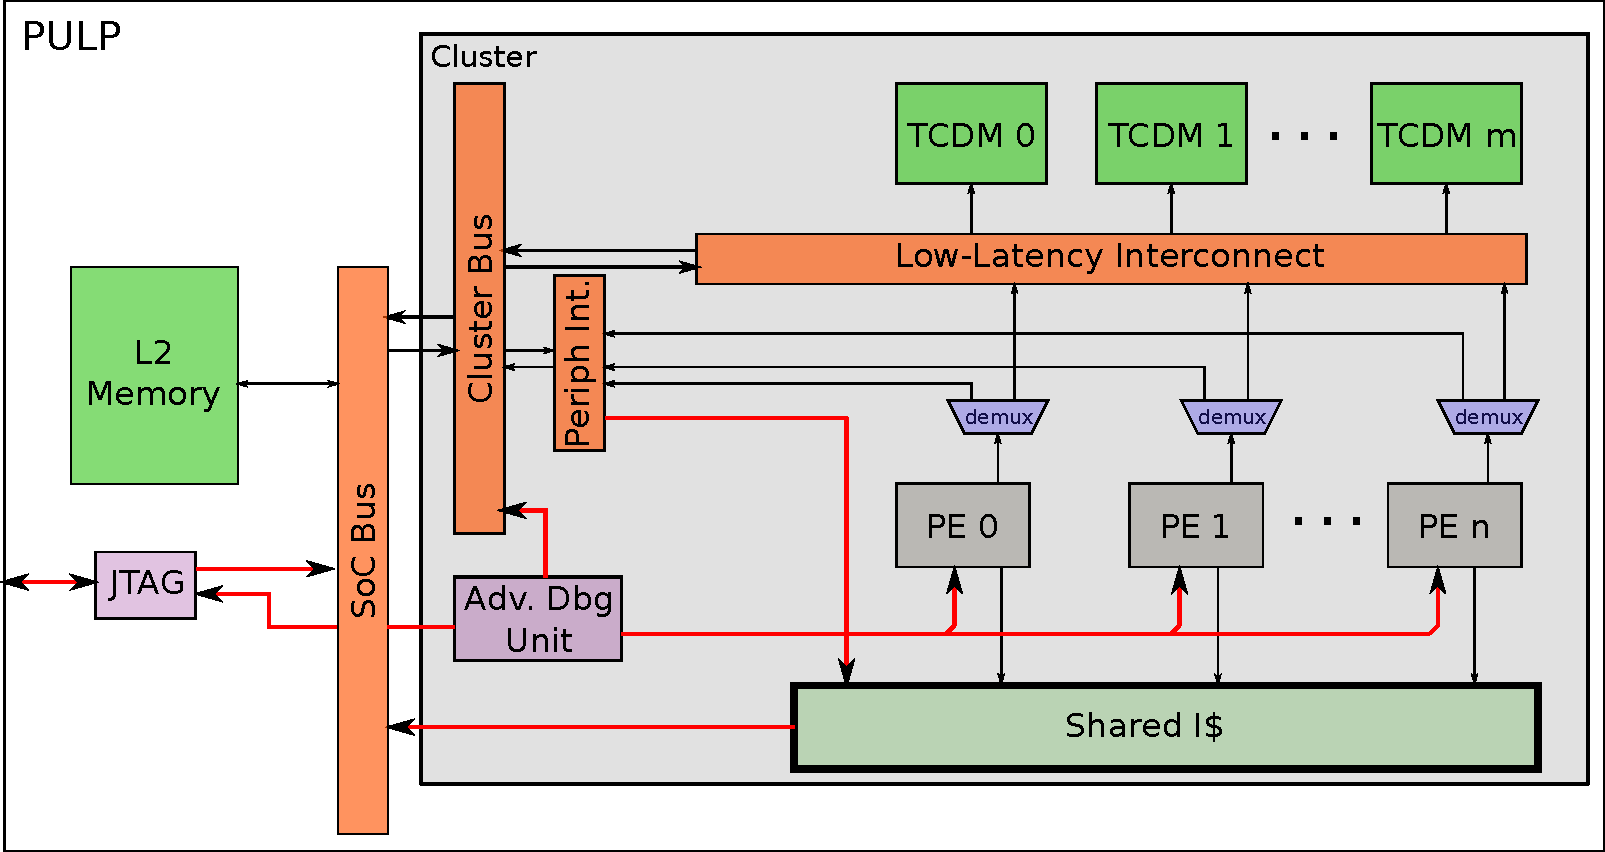
\includegraphics[width=0.9\textwidth]{./figures/debug}
  \caption{PULP debug overview.}
  \label{fig:debug}
\end{figure}
